\documentclass[compress]{beamer}

\usepackage[utf8]{vntex}
\usepackage{longtable,booktabs}
\usepackage{amsmath}
\usepackage{amsfonts}
\usepackage{cases}
\usepackage{amssymb}
\usepackage[utf8]{inputenc}
\usepackage[absolute,overlay]{textpos}
\usepackage{listings}
\usepackage{subcaption}
\usepackage{tikz}
\usepackage{pgfplots}
\usepackage{fancybox}
\usepackage{multicol}
\usepackage{multirow}
\usepackage{tikz-uml}
\tikzumlset{font=\tiny}
\usepackage{movie15}
\usetikzlibrary{arrows.meta}
\usetikzlibrary{shapes.geometric}
\PassOptionsToPackage{hyphens}{url}\usepackage{hyperref}  
\lstset{
	language = Java,
	frame = single,
	tabsize = 3
}

\usetheme{Warsaw}
%\usetheme{Antibes}
%\usecolortheme{spruce}
%\setbeamercolor{structure}{fg=cyan!90!blue}
%\newtheorem{theorem}{Định lý}[]

\expandafter\def\expandafter\insertshorttitle\expandafter{%
    \insertshorttitle\hfill%
    \insertframenumber\,/\,\inserttotalframenumber}
      
\AtBeginSection[] % Do nothing for \section*
{
\begin{frame}
\tableofcontents[currentsection]
\end{frame}
}
\AtBeginSubsection[] % Do nothing for \section*
{
\begin{frame}
\tableofcontents[currentsection, currentsubsection]
\end{frame}
}

\title[Phát triển thuật toán tìm kiếm cục bộ cho bài toán lập lộ trình giao hàng kết hợp xe tải và thiết bị bay drone]{Phát triển thuật toán tìm kiếm cục bộ cho bài toán lập lộ trình giao hàng kết hợp xe tải và thiết bị bay drone} 

\author[Nguyễn Tuấn Đạt]{
Sinh viên thực hiện\\
Nguyễn Tuấn Đạt - 20130856 \\[1em]
Giảng viên hướng dẫn\\
TS. Phạm Quang Dũng}

\begin{document}

\begin{frame}[plain]
\titlepage
\end{frame}

\begin{frame}[plain]{Nội dung trình bày}
\tableofcontents
\end{frame}

\section{Cở sở lý thuyết}
\subsection{Bài toán thỏa mãn ràng buộc}
%\begin{frame}{Một vài khái niêm}
%\begin{block}{Ràng buộc}
%Là một quan hệ trên trên một tập các biến.
%\end{block}
%\begin{block}{Miền giá trị}
%Là một tập hữu hạn các giá trị của biến.
%\end{block}
%\begin{block}{Biểu diễn ràng buộc}
%\begin{itemize}
%\item Biểu thức toán học.
%\item Bảng liệt kê các giá trị phù hợp cho biến.
%\end{itemize}
%\end{block}
%\end{frame}
\begin{frame}{Bài toán thỏa mãn ràng buộc -  Constraint Satisfaction Problem (CSP) }
\begin{block}{Bài toán thỏa mãn ràng buộc}
\begin{enumerate}
\item Một tập các biến X.
\item Tập giá trị (hữu hạn các giá trị) cho mỗi biến D.
\item Một tập hữu hạn các ràng buộc C.
\end{enumerate}
\end{block}
\begin{block}{Lời giải của bài toán CSP}
Là một phép gán giá trị cho tất cả các biến mà thỏa mãn tất cả ràng buộc C.

\end{block}
\begin{alertblock}{Hàm mục tiêu}
Yêu cầu tối ưu một hoặc nhiều hàm mục tiêu.
\end{alertblock}
\end{frame}
\begin{frame}{Ví dụ - N con hậu (N-Queen)}
\begin{exampleblock}{Phát biểu}
\begin{itemize}
\item Xếp n quân hậu trên bàn cờ nxn.
\item Hai quân hậu bất kì không ăn được nhau. 
\end{itemize}
\end{exampleblock}
\end{frame}
\begin{frame}{Ví dụ - N con hậu (N-Queen)}
\begin{block}{Mô hình}
\begin{itemize}
\item Biến $X=\{x_1, x_2, \dots,x_n\}$, $x_i$ - cột của con hậu hàng thứ $i$.
\item Tập giá trị $D(x_i)=\{1,\ldots,n\}, \ \forall i=1,2,\dots,n$
\item Ràng buộc :
\begin{enumerate}


\item 
$ x_i \neq x_j, \ \forall i \neq j, \quad i,j \in \{1,\dots,n\} $
\item 
$x_i-x_j \neq i-j , \ \forall i \neq j, \quad i,j \in \{1,\dots,n\}$
$x_j-x_i \neq i-j, \ \forall i \neq j, \quad i,j \in \{1,\dots,n\}$
\end{enumerate}
\end{itemize}
\end{block}
\begin{exampleblock}{Ví dụ}

\begin{columns}
\begin{column}{0.3\textwidth}
  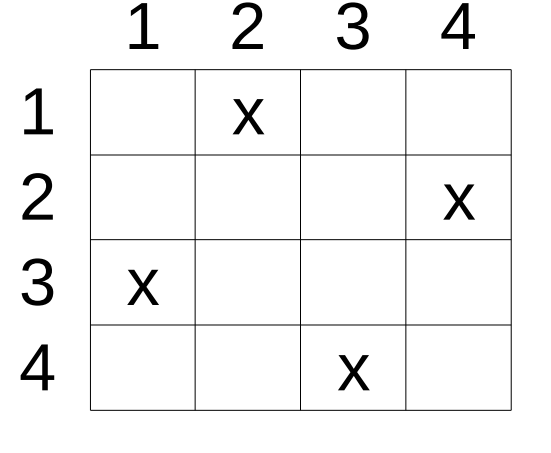
\includegraphics[scale=0.2]{n-queen.png}
\end{column}
\begin{column}{0.7\textwidth}  
     $$x_1=2,x_2=4,x_3=1,x_4=3$$
\end{column}
\end{columns}
\end{exampleblock}
\end{frame}

\subsection{Các hướng tiếp cận giải bài toán thỏa mãn ràng buộc}
\begin{frame}{Các hướng tiếp cận giải bài toán thỏa mãn ràng buộc}
\begin{block}{Thuật toán giải đúng}

\begin{itemize}
\item Quy hoạch động (Dynamic Programming).
\item Quy hoạch ràng buộc (Contraint Programming).
\item Quy hoạch nguyên tuyến tính (Linear Integer Programming).
\end{itemize}

\end{block}
\begin{block}{Thuật toán giải gần đúng}
\begin{itemize}
\item Thuật toán tham lam (Greedy Algorithms).
\item Thuật toán tìm kiếm cục bộ (Local Search Algorithms).
\item Thuật toán di truyền (Genetic Algorithms).
\end{itemize}

\end{block}
\end{frame}
\section{Bài toán lập lộ trình giao hàng kết hợp một xe tải với một thiết bị bay drone}
\subsection{Mô tả bài toán}
\begin{frame}{Mở đầu}
\footnotesize
\begin{longtable}{|l|p{4.2cm}|p{4.2cm}|}
\caption{Bảng thể hiện ưu điểm, nhược điểm của drone và xe tải}
\label{undronexetai}\\
\toprule
&Drone& Xe tải \\
\midrule
\toprule

Ưu điểm & Drone là một phương tiện bay. &Có nhiều năng lượng.\\
& Drone tốn ít chi phí hơn xe tải. &Có thể vận chuyển nhiều hàng hóa.\\
& Drone bay giao hàng nhanh hơn xe tải.&\\
& Drone không cần người lái.&\\
\\
\hline
Nhược điểm & 
 Giới hạn năng lượng. & Phải đi theo mạng lưới đường bộ.\\
& Giới hạn khối lượng.& Phải có người lái. \\
\hline
\end{longtable}
\normalsize
\begin{block}{Bài toán min-cost TSPD [Ha el at. 2017]}
Xe tải và drone cùng giao hàng trên một lộ trình.
\end{block}
\end{frame}
%\begin{frame}{Bài toán min-cost TSPD}
%\begin{block}{Các đặc điểm}
%\begin{itemize}
%\item Đi cùng nhau, cùng tham gia giao hàng.
%\item Điểm bay lên và điểm hạ cánh của drone là khác nhau.
%\item Xe tải không quay lại điểm nó đã đi qua.
%\item \textbf{Hàm mục tiêu:} Tối thiểu chi phí.
%\end{itemize}
%\end{block}
%\end{frame}
\begin{frame}{Bài toán min-cost TSPD}
\begin{block}{Mô tả}
\begin{itemize}
\item[-] Xuất phát và kết thúc chuỗi giao hàng tại kho.
\item[-] Drone cất cánh và hạ cánh từ xe tải.
\item[-] Điểm cất cánh và hạ cánh phải là điểm kho hoặc điểm khách hàng.
\item[-] Chi phí \begin{itemize}
\item Drone - $C_2$/ đơn vị độ dài
\item Xe tải - $C_1$/ đơn vị độ dài.
\end{itemize}
\end{itemize}
\end{block}
\end{frame}
\begin{frame}{Bài toán min-cost TSPD}


\begin{block}{Các ràng buộc}
\begin{itemize}

\item[-] Drone chỉ giao một khách hàng một lượt.
\item[-] Mỗi khách hàng chỉ được giao bởi drone hoặc xe tải và chỉ duy nhất một drone hoặc xe tải.
\item[-] Một drone tại một thời điểm.
\item[-] Drone không được giao hàng quá xa ($\varepsilon$).
\item[-] Thời gian chờ nhau không được vượt quá $\Delta$.


\end{itemize}
\end{block}

\begin{block}{Hàm mục tiêu}

Hàm mục tiêu là tối thiểu tổng chi phí của lộ trình giao hàng.
\end{block}
\end{frame}
\begin{frame}{Một vài định nghĩa}
\begin{block}{Một chuyến giao hàng bởi drone - Drone Delivery (DD)}
$$\langle launch\_node, drone\_node, rendezvous\_node \rangle$$
\begin{itemize}
\item $launch\_node$ - điểm bay của drone.
\item $drone\_node$ - điểm giao hàng.
\item $rendezvous\_node$ - điểm hạ cánh, điểm đón.
\end{itemize}
\end{block}
\begin{block}{Chuyến giao hàng bởi xe tải - Truck Delivery (TD)}
Một chuỗi lộ trình qua các điểm với hai điểm đầu cuối là điểm kho. 

\end{block}
\end{frame}
\begin{frame}
\begin{figure}[H]
\begin{subfigure}{0.45\textwidth}
\begin{tikzpicture}[scale=0.6,every node/.style={scale=0.6},
state/.style ={circle,draw},state1/.style ={circle,dashed,draw},state2/.style={rectangle , draw}]
\node[state2] (1) at (0,0){};
\node[state] (2) at (4,1){6};
\node[state] (3) at (6,2){3};
\node[state] (4) at (5,8){5};
\node[state] (5) at (0,10){2};

\node[state] (6) at (3,4){1};
\node[state] (7) at (2,3){4};
\path [->] (1) edge node[above] {225} (2);
\path [->] (2) edge node[above] {175} (3);
\path [->] (3) edge node[right] {300} (4);
\path [->] (4) edge node[right] {250} (5);
\path [->] (5) edge node[right] {300} (6);
\path [->] (6) edge node[left] {50} (7);
\path [->] (7) edge node[right] {200} (1);
\end{tikzpicture}
\caption{Một hành trình người du lịch}
\label{tsptour}
\end{subfigure}
\begin{subfigure}{0.45\textwidth}
\begin{tikzpicture}[scale=0.6,every node/.style={scale=0.6},
state/.style ={circle,draw},state1/.style ={circle,dashed,draw},state2/.style={rectangle , draw}]
\node[state2] (1) at (0,0){  };
\node[state] (2) at (4,1){6};
\node[state] (3) at (6,2){3};
\node[state] (4) at (5,8){5};
\node[state] (5) at (0,10){2};

\node[state] (6) at (3,4){1};
\node[state] (7) at (2,3){4};
\path [->] (1) edge node[right] {200} (7);
\path [->] (7) edge node[left] {50} (6);
\path [->] (6) edge node[right] {300} (5);
\path [->] (5) edge node[left] {400} (1);

\path [->][dashed] (4) edge node[above] {9.0} (5);
\path [->][dashed] (6) edge node[right] {10} (4);
\path [->][dashed] (3) edge node[above] {8.2} (6);
\path [->][dashed] (7) edge node[above] {9.0} (3);
\path [->][dashed] (2) edge node[above] {6.4} (7);
\path [->][dashed] (1) edge node[above] {8} (2);

\end{tikzpicture}
\caption{Một hành trình TSPD}
\label{tspdtour}
\end{subfigure}
\caption{Lộ trình bài toán TSP và lộ trình bài toán TSPD tương ứng}\label{tsptspd}
\end{figure}
\end{frame}
\subsection{Thuật toán GRASP}
\begin{frame}{Thuật toán GRASP}
\begin{block}{Ý tưởng}
Thuật toán bao gồm 2 bước: 
\begin{enumerate}
\item[-] Thuật toán phân tách.
\item[-] Thuật toán tìm kiếm cục bộ.
\end{enumerate}
\end{block}
\end{frame}
\begin{frame}{Thuật toán phân tách}
\begin{block}{Thuật toán phân tách}
\begin{enumerate}
\item Xây dựng auxiliary graph;
\item Sinh lời giải.
\end{enumerate}
\end{block}
\end{frame}
\begin{frame}{Auxiliary graph}
\begin{block}{Ý nghĩa}
Mỗi cạnh $\langle i$ $j\rangle$ của đồ thị thể hiện lộ trình con từ $i\rightarrow j$ trong lộ trình TSP ban đầu. 
\end{block}
\begin{block}{Chi phí}
\begin{itemize}
\item Nếu $i,$ $j$ liên tiếp nhau 
$$c_{ij}=C_1d_{ij}$$
\item Nếu $i,k$ không liên tiếp mà  $\langle i,j,k \rangle \in P$
$$\begin{array}{l}
c_{ik}=min_{\langle i,j,k \rangle \in P} \ cost(sub(i,k,s))\\+C_1(d_{prev_sj,next_sj}-d_{prev_sj,j}-d_{j,next_sj})+cost(i,j,k)

\end{array}
$$
\item Ngược lại 
$$c_{ik}=+\infty$$
\end{itemize}
\end{block}
\end{frame}
\begin{frame}{Ví dụ}
\begin{figure}
\begin{subfigure}{0.3\textwidth}
\begin{tikzpicture}[scale=0.5,every node/.style={scale=0.5},
state/.style ={circle,draw},state1/.style ={circle,dashed,draw},state2/.style={rectangle , draw}]
\node[state2] (1) at (0,0){};
\node[state] (2) at (4,1){6};
\node[state] (3) at (6,2){3};
\node[state] (4) at (5,8){5};
\node[state] (5) at (0,10){2};

\node[state] (6) at (3,4){1};
\node[state] (7) at (2,3){4};
\path [->] (1) edge node[above] {225} (2);
\path [->] (2) edge node[above] {175} (3);
\path [->] (3) edge node[right] {300} (4);
\path [->] (4) edge node[right] {250} (5);
\path [->] (5) edge node[right] {300} (6);
\path [->] (6) edge node[left] {50} (7);
\path [->] (7) edge node[right] {200} (1);
\end{tikzpicture}
\caption{Một hành trình người du lịch}
\label{tsptour}
\end{subfigure}
\begin{subfigure}{0.65\textwidth}
\begin{tikzpicture}[scale=0.5,every node/.style={scale=0.5},
state/.style ={circle,draw},state1/.style ={circle,dashed,draw}]
\node[state] (0) at (0,0){0};
\node[state] (6) at (2,0){6};
\node[state] (3) at (4,0){3};
\node[state] (5) at (6,0){5};
\node[state] (2) at (8,0){2};
\node[state] (1) at (10,0){1};
\node[state] (4) at (12,0){4};
\node[state] (7) at (14,0){7};
\path [->] (0) edge node[above] {225} (6);
\path [->] (0) edge[bend right=60] node[above] {413} (3);
\path [->] (0) edge[bend right=60] node[above] {$\infty$} (5);
\path [->] (0) edge[bend right=60] node[above] {$\infty$} (2);
\path [->] (0) edge[bend right=60] node[above] {1264} (1);
\path [->] (0) edge[bend right=60] node[above] {1258} (4);
\path [->] (0) edge[bend right=60] node[above] {1464} (7);
\path [->] (6) edge node[above] {175} (3);
\path [->] (6) edge[bend left=60] node[below] {390} (5);
\path [->] (6) edge[bend left=60] node[above] {$\infty$} (2);
\path [->] (6) edge[bend left=60] node[above] {938} (1);
\path [->] (6) edge[bend left=60] node[above] {989} (4);
\path [->] (6) edge[bend left=60] node[above] {1192} (7);
\path [->] (3) edge node[above] {300} (5);
\path [->] (3) edge[bend right=60] node[above] {569} (2);
\path [->] (3) edge[bend right=60] node[above] {$\infty$} (1);
\path [->] (3) edge[bend right=60] node[above] {859} (4);
\path [->] (3) edge[bend right=60] node[above] {1065} (7);
\path [->] (5) edge node[above] {250} (2);
\path [->] (5) edge[bend left=60] node[below] {368} (1);
\path [->] (5) edge[bend left=60] node[above] {419} (4);
\path [->] (5) edge[bend left=60] node[above] {767} (7);
\path [->] (2) edge node[above] {300} (1);
\path [->] (2) edge[bend right=60] node[above] {310} (4);
\path [->] (2) edge[bend right=60] node[above] {516} (7);
\path [->] (1) edge node[above] {50} (4);
\path [->] (1) edge[bend left=60] node[above] {257} (7);
\path [->] (4) edge node[above] {200} (7);

\end{tikzpicture}
\caption{Auxiliary graph cho lộ trình TSP được trình bày trong hình (a)}\label{augraph}
\end{subfigure}
\caption{Một ví dụ về lộ trình và auxiliary graph tương ứng}
\label{vd1}
\end{figure}
\end{frame}
\begin{frame}{Xây dựng lời giải}
\begin{block}{Xây dựng lời giải}
 Auxiliary graph được sử dụng để tính $v_k$ là đường đi ngắn nhất từ kho đến đỉnh $k$.\\
Cụ thể, đặt $v_0=0$ giá trị $v_k$ của mỗi đỉnh được tính bằng: 
$$v_k=min\{v_i+c_{ik}:(i,k) \in A'\} \ \forall k=1,2,\ldots,n+1$$
\end{block}
\end{frame}
\begin{frame}{Ví dụ}
\begin{minipage}{0.3\textwidth}
\footnotesize
\begin{longtable}{p{0.5cm}|p{0.5cm}|p{0.5cm}}
\caption{Bảng quy hoạch động}
\label{qhd1}\\ 
\toprule
Đỉnh & Min cost & Đỉnh kề trước \\
\midrule
\toprule
0&0&-1\\ \hline
6&225&0\\ \hline
3&400&6\\ \hline
5&615&6\\ \hline
2&865&5\\ \hline
1&983&5\\ \hline
4&1033&1\\ \hline
7&1233&4\\ \hline

\end{longtable}
\normalsize
\end{minipage}
\begin{minipage}{0.65\textwidth}
\begin{figure}
\begin{tikzpicture}[scale=0.5,every node/.style={scale=0.5},
state/.style ={circle,draw},state1/.style ={circle,dashed,draw}]
\node[state] (0) at (0,0){0};
\node[state] (6) at (2,0){6};
\node[state] (3) at (4,0){3};
\node[state] (5) at (6,0){5};
\node[state] (2) at (8,0){2};
\node[state] (1) at (10,0){1};
\node[state] (4) at (12,0){4};
\node[state] (7) at (14,0){7};
\path [->] (0) edge[red] node[above] {225} (6);
\path [->] (0) edge[bend right=60] node[above] {413} (3);
\path [->] (0) edge[bend right=60] node[above] {$\infty$} (5);
\path [->] (0) edge[bend right=60] node[above] {$\infty$} (2);
\path [->] (0) edge[bend right=60] node[above] {1264} (1);
\path [->] (0) edge[bend right=60] node[above] {1258} (4);
\path [->] (0) edge[bend right=60] node[above] {1464} (7);
\path [->] (6) edge node[above] {175} (3);
\path [->] (6) edge[red,bend left=60] node[below] {390} (5);
\path [->] (6) edge[bend left=60] node[above] {$\infty$} (2);
\path [->] (6) edge[bend left=60] node[above] {938} (1);
\path [->] (6) edge[bend left=60] node[above] {989} (4);
\path [->] (6) edge[bend left=60] node[above] {1192} (7);
\path [->] (3) edge node[above] {300} (5);
\path [->] (3) edge[bend right=60] node[above] {569} (2);
\path [->] (3) edge[bend right=60] node[above] {$\infty$} (1);
\path [->] (3) edge[bend right=60] node[above] {859} (4);
\path [->] (3) edge[bend right=60] node[above] {1065} (7);
\path [->] (5) edge node[above] {250} (2);
\path [->] (5) edge[red,bend left=60] node[below] {368} (1);
\path [->] (5) edge[bend left=60] node[above] {419} (4);
\path [->] (5) edge[bend left=60] node[above] {767} (7);
\path [->] (2) edge node[above] {300} (1);
\path [->] (2) edge[bend right=60] node[above] {310} (4);
\path [->] (2) edge[bend right=60] node[above] {516} (7);
\path [->] (1) edge[red] node[above] {50} (4);
\path [->] (1) edge[bend left=60] node[above] {257} (7);
\path [->] (4) edge[red] node[above] {200} (7);

\end{tikzpicture}
\caption{Auxiliary graph cho lộ trình TSP được trình bày trong hình \ref{tsptspd}}\label{augraph2}
\end{figure}
\end{minipage}
\end{frame}
\begin{frame}{Xây dựng lời giải}
\begin{block}{Xây dựng lời giải}
\begin{itemize}
\item Tạo các DD còn thiếu.
\item Hình thành TD.
\end{itemize}
\end{block}
\end{frame}
\begin{frame}{Ví dụ}
\begin{figure}
\begin{subfigure}{0.3\textwidth}
\begin{tikzpicture}[scale=0.5,every node/.style={scale=0.5},
state/.style ={circle,draw},state1/.style ={circle,dashed,draw},state2/.style={rectangle , draw}]
\node[state2] (1) at (0,0){};
\node[state] (2) at (4,1){6};
\node[state] (3) at (6,2){3};
\node[state] (4) at (5,8){5};
\node[state] (5) at (0,10){2};

\node[state] (6) at (3,4){1};
\node[state] (7) at (2,3){4};
\path [->] (1) edge node[above] {225} (2);
\path [->] (2) edge node[above] {371} (4);
\path [->] (4) edge node[right] {346} (6);

\path [->] (6) edge node[left] {50} (7);
\path [->] (7) edge node[right] {200} (1);
\path [->][dashed] (4) edge node[right] {10} (5);
\path [->][dashed] (5) edge node[right] {12} (6);
\path [->][dashed] (2) edge node[right] {7} (3);
\path [->][dashed] (3) edge node[right] {12} (4);
\end{tikzpicture}
\caption{Một hành trình TSPD}
\label{tsptour}
\end{subfigure}
\begin{subfigure}{0.65\textwidth}
\begin{tikzpicture}[scale=0.5,every node/.style={scale=0.5},
state/.style ={circle,draw},state1/.style ={circle,dashed,draw}]
\node[state] (0) at (0,0){0};
\node[state] (6) at (2,0){6};
\node[state] (3) at (4,0){3};
\node[state] (5) at (6,0){5};
\node[state] (2) at (8,0){2};
\node[state] (1) at (10,0){1};
\node[state] (4) at (12,0){4};
\node[state] (7) at (14,0){7};
\path [->] (0) edge[red] node[above] {225} (6);
\path [->] (0) edge[bend right=60] node[above] {413} (3);
\path [->] (0) edge[bend right=60] node[above] {$\infty$} (5);
\path [->] (0) edge[bend right=60] node[above] {$\infty$} (2);
\path [->] (0) edge[bend right=60] node[above] {1264} (1);
\path [->] (0) edge[bend right=60] node[above] {1258} (4);
\path [->] (0) edge[bend right=60] node[above] {1464} (7);
\path [->] (6) edge node[above] {175} (3);
\path [->] (6) edge[red,bend left=60] node[below] {390} (5);
\path [->] (6) edge[bend left=60] node[above] {$\infty$} (2);
\path [->] (6) edge[bend left=60] node[above] {938} (1);
\path [->] (6) edge[bend left=60] node[above] {989} (4);
\path [->] (6) edge[bend left=60] node[above] {1192} (7);
\path [->] (3) edge node[above] {300} (5);
\path [->] (3) edge[bend right=60] node[above] {569} (2);
\path [->] (3) edge[bend right=60] node[above] {$\infty$} (1);
\path [->] (3) edge[bend right=60] node[above] {859} (4);
\path [->] (3) edge[bend right=60] node[above] {1065} (7);
\path [->] (5) edge node[above] {250} (2);
\path [->] (5) edge[red,bend left=60] node[below] {368} (1);
\path [->] (5) edge[bend left=60] node[above] {419} (4);
\path [->] (5) edge[bend left=60] node[above] {767} (7);
\path [->] (2) edge node[above] {300} (1);
\path [->] (2) edge[bend right=60] node[above] {310} (4);
\path [->] (2) edge[bend right=60] node[above] {516} (7);
\path [->] (1) edge[red] node[above] {50} (4);
\path [->] (1) edge[bend left=60] node[above] {257} (7);
\path [->] (4) edge[red] node[above] {200} (7);

\end{tikzpicture}
\caption{Auxiliary graph cho lộ trình TSP được trình bày trong hình \ref{tsptspd}}\label{augraph}
\end{subfigure}
\caption{Một ví dụ về lộ trình và auxiliary graph tương ứng}
\label{vd1}
\end{figure}
\end{frame}
\begin{frame}{Tìm kiếm cục bộ}
\begin{block}{Mục đích}
Nhằm cải thiện lời giải được đưa ra bởi thuật toán phân tách.
\end{block}
\end{frame}
\begin{frame}{Toán tử $relocation\_truck$}
\begin{block}{Phạm vi}
Các điểm không thuộc bất kì DD nào.
\end{block}
\begin{block}{Thực hiện}
Di chuyển các nút trong TD.
\end{block}
\begin{figure}[H]

\begin{tikzpicture}[scale=0.5,every node/.style={scale=0.5},
state/.style ={circle,draw},state1/.style ={circle,dashed,draw}]
\node[state] (1) at (0,0){1};
\node[state] (2) at (2,0){2};
\node[state] (3) at (4,-1){3};
\node[state] (4) at (6,1){4};
\node[state] (5) at (8,1){5};
\node[state] (6) at (10,0){6};
\node[state] (7) at (12,0){7};
\node[state] (8) at (14,0){8};
\node[state] (9) at (16,0){9};

\path [-] (1) edge[->] node[above] {} (2);
\path [-] (2) edge[->] node[above] {} (4);
\path [dashed] (2) edge[->] node[above] {} (3);
\path [dashed] (3) edge[->] node[above] {} (4);
\path [-] (4) edge[->] node[above] {} (5);
\path [-] (5) edge[->] node[above] {} (6);
\path [-] (6) edge[->] node[above] {} (7);
\path [-] (7) edge[->] node[above] {} (8);
\path [-] (8) edge[->] node[above] {} (9);

\end{tikzpicture}

\begin{tikzpicture}[scale=0.5,every node/.style={scale=0.5},
state/.style ={circle,draw},state1/.style ={circle,dashed,draw}]
\node[state] (1) at (0,0){1};
\node[state] (2) at (2,0){2};
\node[state] (3) at (4,-1){3};
\node[state] (4) at (6,1){4};
\node[state] (5) at (8,1){5};
\node[state] (6) at (10,0){6};
\node[state] (7) at (12,0){7};
\node[state] (8) at (14,0){8};
\node[state] (9) at (16,0){9};

\path [-] (1) edge[->] node[above] {} (2);
\path [-] (2) edge[->] node[above] {} (4);
\path [dashed] (2) edge[->] node[above] {} (3);
\path [dashed] (3) edge[->] node[above] {} (4);
\path [-] (4) edge[->] node[above] {} (5);
\path [-] (5) edge[->, bend left=40] node[above] {} (8);
\path [-] (8) edge[->, bend right=30] node[above] {} (6);
\path [-] (6) edge[->] node[above] {} (7);
\path [-] (7) edge[->, bend right=30] node[above] {} (9);

\end{tikzpicture}
\caption{Toán tử $truck\_relocation$}\label{opeatorRT}
\end{figure}
\end{frame}
\begin{frame}{Toán tử $drone\_relocation$}
\begin{block}{Phạm vi}
Các điểm giao hàng bởi drone, các điểm không thuộc bất kì DD nào.
\end{block}
\begin{block}{Thực hiện}
Di chuyển điểm giao hàng bởi drone qua điểm bay và điểm đón khác, chuyển điểm giao hàng bởi xe tải thành drone.
\end{block}
\begin{figure}[H]

\begin{tikzpicture}[scale=0.5,every node/.style={scale=0.5},
state/.style ={circle,draw},state1/.style ={circle,dashed,draw}]
\node[state] (1) at (0,0){1};
\node[state] (2) at (2,0){2};
\node[state] (3) at (4,-1){3};
\node[state] (4) at (6,1){4};
\node[state] (5) at (8,1){5};
\node[state] (6) at (10,0){6};
\node[state] (7) at (12,0){7};
\node[state] (8) at (14,0){8};
\node[state] (9) at (16,0){9};

\path [-] (1) edge[->] node[above] {} (2);
\path [-] (2) edge[->] node[above] {} (4);
\path [dashed] (2) edge[->] node[above] {} (3);
\path [dashed] (3) edge[->] node[above] {} (4);
\path [-] (4) edge[->] node[above] {} (5);
\path [-] (5) edge[->] node[above] {} (6);
\path [-] (6) edge[->] node[above] {} (7);
\path [-] (7) edge[->] node[above] {} (8);
\path [-] (8) edge[->] node[above] {} (9);

\end{tikzpicture}

\begin{tikzpicture}[scale=0.5,every node/.style={scale=0.5},
state/.style ={circle,draw},state1/.style ={circle,dashed,draw}]
\node[state] (1) at (0,0){1};
\node[state] (2) at (2,0){2};
\node[state] (3) at (4,-1){3};
\node[state] (4) at (6,1){4};
\node[state] (5) at (8,1){5};
\node[state] (6) at (10,0){6};
\node[state] (7) at (12,0){7};
\node[state] (8) at (14,0){8};
\node[state] (9) at (16,0){9};

\path [-] (1) edge[->] node[above] {} (2);
\path [-] (2) edge[->] node[above] {} (4);
\path [dashed] (2) edge[->] node[above] {} (3);
\path [dashed] (3) edge[->] node[above] {} (4);
\path [-][dashed] (4) edge[->] node[above] {} (5);
\path [-][dashed] (5) edge[->] node[above] {} (6);
\path [-] (4) edge[->] node[above] {} (6);
\path [-] (6) edge[->] node[above] {} (7);
\path [-] (7) edge[->] node[above] {} (8);
\path [-] (8) edge[->] node[above] {} (9);

\end{tikzpicture}
\caption{Toán tử $drone\_relocation$}\label{opeatorRD}
\end{figure}
\end{frame}
\begin{frame}{Toán tử $drone\_removal$}
\begin{block}{Phạm vi}
Các điểm giao hang bởi drone.
\end{block}
\begin{block}{Thực hiện}
Xóa bỏ DD chuyển thành giao hàng bằng xe tải.
\end{block}
\begin{figure}[H]

\begin{tikzpicture}[scale=0.5,every node/.style={scale=0.5},
state/.style ={circle,draw},state1/.style ={circle,dashed,draw}]
\node[state] (1) at (0,0){1};
\node[state] (2) at (2,0){2};
\node[state] (3) at (4,-1){3};
\node[state] (4) at (6,1){4};
\node[state] (5) at (8,1){5};
\node[state] (6) at (10,0){6};
\node[state] (7) at (12,0){7};
\node[state] (8) at (14,0){8};
\node[state] (9) at (16,0){9};

\path [-] (1) edge[->] node[above] {} (2);
\path [-] (2) edge[->] node[above] {} (4);
\path [dashed] (2) edge[->] node[above] {} (3);
\path [dashed] (3) edge[->] node[above] {} (4);
\path [-] (4) edge[->] node[above] {} (5);
\path [-] (5) edge[->] node[above] {} (6);
\path [-] (6) edge[->] node[above] {} (7);
\path [-] (7) edge[->] node[above] {} (8);
\path [-] (8) edge[->] node[above] {} (9);

\end{tikzpicture}

\begin{tikzpicture}[scale=0.5,every node/.style={scale=0.5},
state/.style ={circle,draw},state1/.style ={circle,dashed,draw}]
\node[state] (1) at (0,0){1};
\node[state] (2) at (2,0){2};
\node[state] (3) at (4,-1){3};
\node[state] (4) at (6,1){4};
\node[state] (5) at (8,1){5};
\node[state] (6) at (10,0){6};
\node[state] (7) at (12,0){7};
\node[state] (8) at (14,0){8};
\node[state] (9) at (16,0){9};

\path [-] (1) edge[->] node[above] {} (2);
\path [-] (2) edge[->] node[above] {} (3);
\path [-] (3) edge[->] node[above] {} (4);
\path [-] (4) edge[->] node[above] {} (5);
\path [-] (5) edge[->] node[above] {} (6);
\path [-] (6) edge[->] node[above] {} (7);
\path [-] (7) edge[->] node[above] {} (8);
\path [-] (8) edge[->] node[above] {} (9);

\end{tikzpicture}
\caption{Toán tử $drone\_removal$}\label{opeatorDR}
\end{figure}
\end{frame}
\begin{frame}{Toán tử $two\_exchange$}
\begin{block}{Phạm vi}
\begin{itemize}
\item Hai điểm giao hàng bởi drone.
\item Hai điểm giao hàng bởi xe tải.
\item Một điểm giao hàng bởi xe tải và drone.
\end{itemize}
\end{block}
\begin{block}{Thực hiện}
Đổi vị trí hai điểm.
\end{block}
\begin{figure}[H]

\begin{tikzpicture}[scale=0.5,every node/.style={scale=0.5},
state/.style ={circle,draw},state1/.style ={circle,dashed,draw}]
\node[state] (1) at (0,0){1};
\node[state] (2) at (2,0){2};
\node[state] (3) at (4,-1){3};
\node[state] (4) at (6,1){4};
\node[state] (5) at (8,1){5};
\node[state] (6) at (10,0){6};
\node[state] (7) at (12,0){7};
\node[state] (8) at (14,0){8};
\node[state] (9) at (16,0){9};

\path [-] (1) edge[->] node[above] {} (2);

\path [-] (2) edge[->] node[above] {} (3);
\path [-] (3) edge[->] node[above] {} (4);
\path [dashed] (4) edge[->] node[above] {} (5);
\path [dashed] (5) edge[->] node[above] {} (6);
\path [-] (4) edge[->] node[above] {} (6);
\path [-] (6) edge[->] node[above] {} (7);
\path [-] (7) edge[->] node[above] {} (8);
\path [-] (8) edge[->] node[above] {} (9);

\end{tikzpicture}

\begin{tikzpicture}[scale=0.5,every node/.style={scale=0.5},
state/.style ={circle,draw},state1/.style ={circle,dashed,draw}]
\node[state] (1) at (0,0){1};
\node[state] (2) at (2,0){2};
\node[state] (3) at (4,-1){3};
\node[state] (4) at (6,1){4};
\node[state] (5) at (8,1){5};
\node[state] (6) at (10,0){6};
\node[state] (7) at (12,0){7};
\node[state] (8) at (14,0){8};
\node[state] (9) at (16,0){9};

\path [-] (1) edge[->] node[above] {} (2);
\path [-] (2) edge[->,bend left=45] node[above] {} (5);
\path [-] (5) edge[->] node[above] {} (4);
\path [dashed] (4) edge[->] node[above] {} (3);
\path [dashed] (3) edge[->] node[above] {} (6);
\path [-] (4) edge[->] node[above] {} (6);
\path [-] (6) edge[->] node[above] {} (7);
\path [-] (7) edge[->] node[above] {} (8);
\path [-] (8) edge[->] node[above] {} (9);

\end{tikzpicture}
\caption{Toán tử $two\_exchange$}\label{opeatorTE}
\end{figure}
\end{frame}
\subsection{Thuật toán TSP-LS}
\begin{frame}{Thuật toán TSP-LS}
\begin{block}{Ý tưởng}
Lặp đi lặp lại hai thao tác :
\begin{itemize}
\item relocateAsTruck - cập nhật lại vị trí của các điểm trong TD. 
\item relocateAsDrone - chuyển một điểm giao hàng bằng xe tải thành drone.
\end{itemize}
đến khi chi phí không giảm được nữa.
\end{block}
\end{frame}
\begin{frame}{Mô phỏng hai thao tác}
\begin{figure}[H]
\begin{tikzpicture}[scale=0.7,every node/.style={scale=0.7},
state/.style ={circle,draw},state1/.style ={circle,dashed,draw}]
\node[state] (1) at (0,0){1};
\node[state] (2) at (2,0){2};
\node[state] (3) at (4,-1){3};
\node[state1] (4) at (6,1){4};
\node[state] (5) at (8,1){5};
\node[state] (6) at (10,0){6};
\node[state] (7) at (12,0){7};
\node[state] (8) at (14,0){8};
\node[state] (9) at (16,0){9};

\path [->] (1) edge node[above] {} (2);
\path [->] (2) edge node[above] {} (3);
\path [->] (3) edge node[above] {} (5);
\path [->,dashed] (3) edge node[above] {} (4);
\path [->,dashed] (4) edge node[above] {} (5);
\path [->] (5) edge node[above] {} (6);
\path [->] (6) edge node[above] {} (7);
\path [->] (7) edge node[above] {} (8);
\path [->] (8) edge node[above] {} (9);

\end{tikzpicture}
\begin{tikzpicture}[scale=0.7,every node/.style={scale=0.7},
state/.style ={circle,draw},state1/.style ={circle,dashed,draw}]
\node[state] (1) at (0,0){1};
\node[state] (2) at (2,0){2};
\node[state] (3) at (4,-1){3};
\node[state1] (4) at (6,1){4};
\node[state] (5) at (8,1){5};
\node[state] (6) at (10,0){6};
\node[state] (7) at (12,0){7};
\node[state] (8) at (14,0){8};
\node[state] (9) at (16,0){9};

\path [->] (1) edge node[above] {} (2);
\path [->] (2) edge node[above] {} (3);
\path [->] (3) edge[bend right=45] node[above] {} (7);
\path [->,dashed] (3) edge node[above] {} (4);
\path [->,dashed] (4) edge node[above] {} (5);
\path [->] (7) edge[bend left=45] node[above] {} (5);
\path [->] (5) edge node[above] {} (6);
\path [->] (6) edge[bend left=45] node[above] {} (8);
\path [->] (8) edge node[above] {} (9);

\end{tikzpicture}
\caption{Mô phỏng thao tác relocateAsTruck}\label{reloAsTruck}
\end{figure}

\end{frame}
\begin{frame}{Mô phỏng hai thao tác}

\begin{figure}[H]
\begin{tikzpicture}[scale=0.7,every node/.style={scale=0.7},
state/.style ={circle,draw},state1/.style ={circle,dashed,draw}]
\node[state] (1) at (0,0){1};
\node[state] (2) at (2,0){2};
\node[state] (3) at (4,-1){3};
\node[state1] (4) at (6,1){4};
\node[state] (5) at (8,1){5};
\node[state] (6) at (10,0){6};
\node[state] (7) at (12,0){7};
\node[state] (8) at (14,0){8};
\node[state] (9) at (16,0){9};

\path [->] (1) edge node[above] {} (2);
\path [->] (2) edge node[above] {} (3);
%\path [-] (3) edge node[above] {} (5);
\path [->] (3) edge node[above] {} (4);
\path [->] (4) edge node[above] {} (5);
\path [->] (5) edge node[above] {} (6);
\path [->] (6) edge node[above] {} (7);
\path [->] (7) edge node[above] {} (8);
\path [->] (8) edge node[above] {} (9);

\end{tikzpicture}
\begin{tikzpicture}[scale=0.7,every node/.style={scale=0.7},
state/.style ={circle,draw},state1/.style ={circle,dashed,draw}]
\node[state] (1) at (0,0){1};
\node[state] (2) at (2,0){2};
\node[state] (3) at (4,-1){3};
\node[state1] (4) at (6,1){4};
\node[state] (5) at (8,1){5};
\node[state] (6) at (10,0){6};
\node[state] (7) at (12,0){7};
\node[state] (8) at (14,0){8};
\node[state] (9) at (16,0){9};

\path [->] (1) edge node[above] {} (2);
\path [->] (2) edge node[above] {} (3);
\path [->] (3) edge node[above] {} (5);
\path [->, dashed] (3) edge node[above] {} (4);
\path [->, dashed] (4) edge node[above] {} (5);
\path [->] (5) edge node[above] {} (6);
\path [->] (6) edge node[above] {} (7);
\path [->] (7) edge node[above] {} (8);
\path [->] (8) edge node[above] {} (9);

\end{tikzpicture}
\caption{Mô phỏng thao tác relocateAsDrone}\label{reloAsDrone}
\end{figure}
\end{frame}
\section{Đề xuất thuật toán tìm kiếm cục bộ giải bài toán lập lộ trình giao hàng kết hợp xe tải và nhiều thiết bị bay drone}
\begin{frame}{ Bài toán lập lộ trình giao hàng kết hợp xe tải và nhiều thiết bị bay drone}
\begin{block}{Nhận xét}
Dựa vào các ưu nhược điểm của xe tải và drone được đưa ra vào phần trước. 
\begin{itemize}
\item Sử dụng thêm drone có thể giảm chi phí nhiều hơn một drone.
\item Xe tải với năng lực của nó có thể mang nhiều hơn 1 drone.
\end{itemize}
\end{block}
\end{frame}
\subsection{Giới thiệu bài toán}
\begin{frame}{Bài toán min-cost TSPkD}
\begin{block}{Mô tả}
\begin{itemize}
\item[-] Xuất phát và kết thúc chuỗi giao hàng tại kho.
\item[-] Drone cất cánh và hạ cánh từ xe tải.
\item[-] Điểm cất cánh và hạ cánh phải là điểm kho hoặc điểm khách hàng.
\item[-] Chi phí \begin{itemize}
\item Drone - $C_2$/ đơn vị độ dài
\item Xe tải - $C_1$/ đơn vị độ dài.
\end{itemize}
\item Xe tải cần đợi tất cả drone quay về trước khi bắt đầu thực hiện chuyến giao hàng mới hoặc thả drone thực hiện chuyến giao hàng mới.
\item Các drone xuất phát ở cùng một điểm thì coi như xuất phát cùng lúc
\end{itemize}
\end{block}
\end{frame}
\begin{frame}{Bài toán min-cost TSPkD}


\begin{block}{Các ràng buộc}
\begin{itemize}

\item[-] Drone chỉ giao một khách hàng một lượt.
\item[-] Mỗi khách hàng chỉ được giao bởi drone hoặc xe tải và chỉ duy nhất một drone hoặc xe tải.
\item[-] K drone tại một thời điểm.
\item[-] Drone không được giao hàng quá xa ($\varepsilon$).
\item[-] Thời gian chờ nhau không được vượt quá $\Delta$.


\end{itemize}
\end{block}

\begin{block}{Hàm mục tiêu}

Hàm mục tiêu là tối thiểu tổng chi phí của lộ trình giao hàng.
\end{block}
\end{frame}
\subsection{Toán tử}
\begin{frame}{Ví dụ}
\begin{figure}[H]
\begin{subfigure}{1\textwidth}
\begin{tikzpicture}[scale=0.55,every node/.style={scale=0.55},
state/.style ={circle,draw},state1/.style ={circle,dashed,draw}]
\node[state] (1) at (0,0){1};
\node[state] (2) at (2,0){2};
\node[state] (3) at (4,0){3};
\node[state] (4) at (6,2){4};
\node[state] (5) at (8,2){5};
\node[state] (6) at (10,0){6};
\node[state] (7) at (12,0){7};
\node[state] (8) at (14,0){8};
\node[state] (9) at (16,0){9};

\path [-] (1) edge[->] node[above] {} (2);
\path [-] (2) edge[->] node[above] {} (3);
\path [-] (3) edge[->] node[above] {} (4);
\path [-] (4) edge[->] node[above] {} (5);
\path [-] (5) edge[->] node[above] {} (6);
\path [-] (6) edge[->] node[above] {} (7);
\path [-] (7) edge[->] node[above] {} (8);
\path [-] (8) edge[->] node[above] {} (9);

\end{tikzpicture}
\caption{Lộ trình TSP ban đầu}
\label{exTSPkD1}
\end{subfigure}
\begin{subfigure}{1\textwidth}
\begin{tikzpicture}[scale=0.55,every node/.style={scale=0.55},
state/.style ={circle,draw},state1/.style ={circle,dashed,draw}]
\node[state] (1) at (0,0){1};
\node[state] (2) at (2,0){2};
\node[state] (3) at (4,0){3};
\node[state1] (4) at (6,2){4};
\node[state] (5) at (8,2){5};
\node[state] (6) at (10,0){6};
\node[state] (7) at (12,0){7};
\node[state] (8) at (14,0){8};
\node[state] (9) at (16,0){9};

\path [-] (1) edge[->] node[above] {} (2);
\path [-] (2) edge[->] node[above] {} (3);
\path [dashed] (3) edge[->] node[above] {} (4);
\path [dashed] (4) edge[->] node[above] {} (5);
\path [-] (3) edge[->] node[above] {} (5);
\path [-] (5) edge[->] node[above] {} (6);
\path [-] (6) edge[->] node[above] {} (7);
\path [-] (7) edge[->] node[above] {} (8);
\path [-] (8) edge[->] node[above] {} (9);

\end{tikzpicture}
\caption{Lời giải ứng với toán tử $relocation_D$}
\label{exTSPkD2}
\end{subfigure}
\begin{subfigure}{1\textwidth}
\begin{tikzpicture}[scale=0.55,every node/.style={scale=0.55},
state/.style ={circle,draw},state1/.style ={circle,dashed,draw}]
\node[state] (1) at (0,0){1};
\node[state] (2) at (2,0){2};
\node[state] (3) at (4,0){3};
\node[state1] (4) at (6,2){4};
\node[state1] (5) at (8,2){5};
\node[state] (6) at (10,0){6};
\node[state] (7) at (12,0){7};
\node[state] (8) at (14,0){8};
\node[state] (9) at (16,0){9};

\path [-] (1) edge[->] node[above] {} (2);
\path [-] (2) edge[->] node[above] {} (3);
\path [-] (3) edge[->] node[above] {} (6);
\path [dashed] (3) edge[->] node[above] {} (4);
\path [dashed] (4) edge[->] node[above] {} (6);
\path [dashed] (3) edge[->] node[above] {} (5);
\path [dashed] (5) edge[->] node[above] {} (6);
\path [-] (6) edge[->] node[above] {} (7);
\path [-] (7) edge[->] node[above] {} (8);
\path [-] (8) edge[->] node[above] {} (9);

\end{tikzpicture}
\label{exTSPkD3}
\caption{Lời giải đúng cho bài toán min cost TSPkD}
\end{subfigure}
\caption{Ví dụ cho thao tác $relocate_D$ sang bài toán min-cost TSPkD}\label{exTSPkD}
\end{figure}
\end{frame}
\begin{frame}{Toán tử move-$t$-point}
\begin{block}{Thực hiện}
\begin{itemize}
\item[-] Bước 1: Chọn $t$ điểm giao hàng liên tiếp trong lộ trình $\langle v_1,v_2,\ldots,v_t \rangle$
\item[-] Bước 2: Xóa bỏ $t$ điểm giao hàng vừa chọn ra khỏi lộ trình.
\item[-] Bước 3: Với mỗi $v_i$ ta thực hiện các bước: 
\begin{enumerate}
\item Tìm hai điểm $v_{il}$ $v_{ir}$ trong lộ trình sao cho lượng chi phí giảm được nhiều nhất.
\item Tạo DD mới với $v_{il}$ $v_{i}$ $v_{ir}$
\end{enumerate}
\end{itemize}
\end{block}
\end{frame}
\begin{frame}{Mô phỏng thao tác move-$t$-point}

\begin{figure}[H]

\begin{tikzpicture}[scale=0.55,every node/.style={scale=0.55},
state/.style ={circle,draw},state1/.style ={circle,dashed,draw}]
\node[state] (1) at (0,0){1};
\node[state] (2) at (2,0){2};
\node[state1] (3) at (4,-1){3};
\node[state1] (4) at (6,1){4};
\node[state1] (5) at (8,1){5};
\node[state] (6) at (10,0){6};
\node[state] (7) at (12,0){7};
\node[state] (8) at (14,0){8};
\node[state] (9) at (16,0){9};

\path [-] (1) edge[->] node[above] {} (2);
\path [-] (2) edge[->] node[above] {} (3);
\path [-] (3) edge[->] node[above] {} (4);
\path [-] (4) edge[->] node[above] {} (5);
\path [-] (5) edge[->] node[above] {} (6);
\path [-] (6) edge[->] node[above] {} (7);
\path [-] (7) edge[->] node[above] {} (8);
\path [-] (8) edge[->] node[above] {} (9);

\end{tikzpicture}


\begin{tikzpicture}[scale=0.55,every node/.style={scale=0.55},
state/.style ={circle,draw}]
\node[state] (1) at (0,0){1};
\node[state] (2) at (2,0){2};
\node[state] (3) at (4,-1){3};
\node[state] (4) at (6,1){4};
\node[state] (5) at (8,1){5};
\node[state] (6) at (10,0){6};
\node[state] (7) at (12,0){7};
\node[state] (8) at (14,0){8};
\node[state] (9) at (16,0){9};

\path [-] (1) edge[->] node[above] {} (2);
\path [-] (2) edge[->] node[above] {} (6);

\path [-] (6) edge[->] node[above] {} (7);
\path [-] (7) edge[->] node[above] {} (8);
\path [-] (8) edge[->] node[above] {} (9);

\end{tikzpicture}


\begin{tikzpicture}[scale=0.55,every node/.style={scale=0.55},
state/.style ={circle,draw}]
\node[state] (1) at (0,0){1};
\node[state] (2) at (2,0){2};
\node[state] (3) at (4,-1){3};
\node[state] (4) at (6,1){4};
\node[state] (5) at (8,1){5};
\node[state] (6) at (10,0){6};
\node[state] (7) at (12,0){7};
\node[state] (8) at (14,0){8};
\node[state] (9) at (16,0){9};

\path [-] (1) edge[->] node[above] {} (2);
\path [-] (2) edge[->] node[above] {} (6);
\path [dashed] (2) edge[->] node[above] {} (3);
\path [dashed] (3) edge[->] node[above] {} (6);
\path [dashed] (2) edge[->] node[above] {} (4);
\path [dashed] (4) edge[->] node[above] {} (6);
\path [dashed] (7) edge[->, bend right=10] node[above] {} (5);
\path [dashed]  (5) edge[->, bend left=30] node[above] {} (8);

\path [-] (6) edge[->] node[above] {} (7);
\path [-] (7) edge[->] node[above] {} (8);
\path [-] (8) edge[->] node[above] {} (9);

\end{tikzpicture}
\caption{Mô phỏng thao tác move-$3$-point}\label{mov3point3}
\end{figure}
\end{frame}
\subsection{Thuật toán tìm kiếm cục bộ}
\begin{frame}{Ý tưởng}

\begin{block}{Ý tưởng}
Với một lần lặp các thao tác move
\begin{itemize}
\item $relocate_T$
\item $relocate_D$
\item $remove_D$
\item $two\_exchange$
\item $move\_t\_point$
\end{itemize}
được đưa ra tính toán chi phí. Toán tử move cho chi phí giảm nhiều nhất được chọn. Thuật toán dừng lại khi không còn toán tử move nào cho chi phí giảm.
\end{block}

\end{frame}
\section{Thực nghiệm và đánh giá}
\subsection{Dữ liệu}
\begin{frame}{Dữ liệu}
\footnotesize
\begin{longtable}{|l|p{4.25cm}|p{4.25cm}|}
\caption{Bảng thể hiện thông số bộ dữ liệu 1,2}
\label{data}\\
\toprule
&Bộ dữ liệu 1 & Bộ dữ liêu 2\\
\midrule
\toprule
Dữ liệu &Bao gồm 35 tập dữ liệu với số điểm là 10 và 50. \newline Chú ý: Bộ dữ liệu có định nghĩa sẵn tập điểm giao hàng mà được phép giao hàng bởi drone. &Bao gồm 10 tập dữ liệu với số điểm lần lượt 10, 20, 30, 40, 50, tương ứng một số điểm có 2 tập dữ liệu. \\
\hline
Khoảng cách & Drone : Euclide \newline Xe tải : Manhattan & Drone : Euclide \newline Xe tải : GoogleMap\\
\hline
\end{longtable}
\normalsize
\begin{block}{Các tham số chung}
\begin{multicols}{2}
\begin{itemize}
\item TruckSpeed: 40 km/h
\item DroneSpeed: 40 km/h
\item TruckCost: 25/1km
\item DroneCost: 1/1km
\item $\Delta$: 15 phút
\item $\varepsilon$: 15 km
\end{itemize}
\end{multicols}

\end{block}

\end{frame}
%\begin{frame}{Dữ liệu}
%\begin{block}{Bộ 2}
%
%\begin{itemize}
%\item Tốc độ của xe tải: 40 km/h
%\item Tốc độ của drone: 40 km/h
%\item Chi phí trên 1km của xe tải: 25
%\item Chi phí trên 1km của drone: 1
%\item Khoảng thời gian tối đa hai phương tiện đợi nhau: 15 phút
%\item Sức chịu đựng của drone: 15 km
%\item Bao gồm 10 tập dữ liệu với số điểm lần lượt 10, 20, 30, 40, 50, tương ứng một số điểm có 2 tập dữ liệu. 
%\end{itemize}
%
%\end{block}
%\end{frame}
\subsection{Kết quả thử nghiệm}
\begin{frame}{Môi trường thực nghiệm}
Thuật toán được cài đặt bằng ngôn ngữ lập trình Java, chạy trên máy sử dụng hệ điều hành Window, cấu hình máy :
\begin{itemize}
\item CPU: Intel Core i5-2520M CPU @ 2,25 GHz.
\item Memory: 8Gb.
\end{itemize}
Trong thực nghiệm chúng tôi chọn bộ tham số như sau : 
\begin{itemize}
\item Với thư viện CBLSVR: \begin{itemize}
\item MaxStable 50
\item MaxIter 300
\item TimeLimit 10
\end{itemize}
\item Với TSPkD : \begin{itemize}
\item maxRangeMove 7
\end{itemize}
\end{itemize}
\end{frame}
\begin{frame}{Bộ dữ liệu 1}
\tiny
\begin{longtable}{|p{0.2cm}|p{1.0cm}|p{0.55cm}|p{0.85cm}|p{0.6cm}|p{0.7cm}|c|p{0.85cm}|c|p{0.85cm}|}
\caption{Bảng kết quả bộ dữ liệu 1 ứng với 1, 2, 3, 4 drones}
\label{tabletspkd1}\\ 
\toprule
STT&\multirow{2}{*}{Tập dữ liệu} & \multicolumn{2}{c|}{tspd-1-drone } &\multicolumn{2}{c|}{tspd-2-drone } &\multicolumn{2}{c|}{tspd-3-drone }&\multicolumn{2}{c|}{tspd-4-drone } \\
\cline{3-10} 
&&Chi phí &Thời gian (ms)&Chi phí &Thời gian (ms)&Chi phí &Thời gian (ms)&Chi phí &Thời gian (ms)\\
\midrule
        \toprule
0&$mbA101$ &     990.53 &      1.00 &     990.53 &       0.00 &     990.53 &       1.00 &     990.53 &       0.00\\ \hline 
1&$mbA102$ &     953.64 &      3.00 &     953.64 &       0.00 &     953.64 &       1.00 &     953.64 &       0.00\\ \hline 
2&$mbA103$ &     985.68 &      1.00 &     985.68 &       0.00 &     985.68 &       1.00 &     985.68 &       0.00\\ \hline 
3&$mbA104$ &     911.87 &      1.00 &     911.87 &       1.00 &     911.87 &       0.00 &     911.87 &       1.00\\ \hline 
4&$mbA105$ &     911.67 &      2.00 &     910.55 &       0.00 &     910.55 &       1.00 &     910.55 &       0.00\\ \hline 
5&$mbB101$ &    2086.51 & 228515.00 &    2099.51 &     488.00 &    2099.51 &     286.00 &    2099.51 &     382.00\\ \hline 
6&$mbB102$ &    1943.58 & 641944.00 &    1958.00 &     264.00 &    1958.00 &     308.00 &    1958.00 &     276.00\\ \hline 
7&$mbB103$ &    1925.97 & 471074.00 &    1872.30 &     350.00 &    1871.79 &     465.00 &    1871.10 &     480.00\\ \hline 
8&$mbB104$ &    2160.91 & 160644.00 &    2122.00 &      57.00 &    2122.00 &      68.00 &    2122.00 &      81.00\\ \hline 
9&$mbB105$ &    1983.99 & 378731.00 &    1969.16 &     148.00 &    1969.16 &     123.00 &    1969.16 &     126.00\\ \hline 
10&$mbB106$ &    2081.65 & 322429.00 &    2081.65 &      83.00 &    2081.65 &      80.00 &    2081.65 &      90.00\\ \hline 
11&$mbB107$ &    2066.85 & 253436.00 &    2064.72 &     248.00 &    2064.72 &     298.00 &    2064.72 &     293.00\\ \hline 
12&$mbB108$ &    2013.60 & 475925.00 &    1969.65 &     220.00 &    1969.65 &     242.00 &    1969.65 &     243.00\\ \hline 
13&$mbB109$ &    1967.11 &1026864.00 &    1946.92 &     298.00 &    1946.92 &     293.00 &    1946.92 &     295.00\\ \hline 
14&$mbB110$ &    2047.90 & 177981.00 &    1947.27 &     367.00 &    1947.57 &     350.00 &    1945.99 &     375.00\\ \hline 
15&$mbC101$ &    3964.19 &   8536.00 &    3963.72 &      61.00 &    3963.72 &      82.00 &    3963.72 &      83.00\\ \hline 
16&$mbC102$ &    3732.77 &   6601.00 &    3732.77 &     160.00 &    3732.77 &     182.00 &    3732.77 &     166.00\\ \hline 
17&$mbC103$ &    3713.82 &  15427.00 &    3661.81 &     417.00 &    3661.81 &     490.00 &    3661.81 &     450.00\\ \hline 
18&$mbC104$ &    4103.35 &  11749.00 &    4058.82 &     184.00 &    4058.82 &     233.00 &    4058.82 &     224.00\\ \hline 
%19&$mbC105$ &    3848.47 &  23550.00 &    3676.27 &     606.00 &    3664.47 &     662.00 &    3664.47 &     892.00\\ \hline 
%20&$mbC106$ &    4041.45 &  22180.00 &    3957.82 &     491.00 &    3957.82 &     354.00 &    3957.82 &     354.00\\ \hline 
%21&$mbC107$ &    4146.52 &  10660.00 &    4145.69 &     109.00 &    4145.69 &     140.00 &    4145.69 &     146.00\\ \hline 
%22&$mbC108$ &    3924.68 &  26514.00 &    3876.36 &     316.00 &    3874.41 &     359.00 &    3874.41 &     439.00\\ \hline 
%23&$mbC109$ &    4044.95 &  17850.00 &    3895.35 &     246.00 &    3894.37 &     262.00 &    3894.37 &     305.00\\ \hline 
%24&$mbC110$ &    3876.91 &  18155.00 &    3870.08 &     141.00 &    3870.08 &     166.00 &    3870.08 &     160.00\\ \hline 
%25&$mbD101$ &    5559.54 &   7470.00 &    5546.41 &     216.00 &    5546.41 &     338.00 &    5546.41 &     292.00\\ \hline 
%26&$mbD102$ &    6033.59 &   3932.00 &    6069.41 &     108.00 &    6069.41 &     142.00 &    6069.41 &     146.00\\ \hline 
%27&$mbD103$ &    5603.71 &   5648.00 &    5603.71 &     311.00 &    5603.71 &     241.00 &    5603.71 &     234.00\\ \hline 
%28&$mbD104$ &    5704.79 &  13405.00 &    5432.29 &     527.00 &    5432.29 &     752.00 &    5432.29 &     711.00\\ \hline 
%29&$mbD105$ &    5726.94 &   4721.00 &    5726.94 &      97.00 &    5726.94 &     108.00 &    5726.94 &     102.00\\ \hline 
%30&$mbD106$ &    5561.71 &   9631.00 &    5561.71 &     425.00 &    5561.71 &     356.00 &    5561.71 &     366.00\\ \hline 
%31&$mbD107$ &    5869.62 &   3879.00 &    5867.98 &     110.00 &    5867.98 &     113.00 &    5867.98 &     110.00\\ \hline 
%32&$mbD108$ &    5193.21 &   9347.00 &    5187.36 &     355.00 &    5179.85 &     415.00 &    5179.85 &     509.00\\ \hline 
%33&$mbD109$ &    5990.58 &   6391.00 &    5891.65 &     177.00 &    5851.43 &     326.00 &    5851.43 &     414.00\\ \hline 
%34&$mbD110$ &    5518.99 &   4487.00 &    5308.85 &     141.00 &    5308.85 &     136.00 &    5308.85 &     143.00\\ \hline 

\end{longtable}
\begin{center}


(\ldots  còn 16 hàng nữa )
\end{center}
\normalsize
\end{frame}
\begin{frame}{Bộ dữ liệu 1}
\begin{figure}

\begin{tikzpicture}[scale=0.7]
\begin{axis}[
    title={Biểu đồ thể hiện kết quả của k drone so với một drone (Bộ dữ liệu 1)},
    xlabel={Bộ dữ liệu},
    ylabel={\% Chênh lệch so với kết quả tspd 1 drone},
    xmin=0, xmax=35,
    ymin=-6, ymax=5,
    xtick={0,5,10,15,20,25,30,35},
    ytick={-6,-5,-4,-3,-2,-1,0,1,2,3,4,5},
    legend pos=north west,
    ymajorgrids=true,
    grid style=dashed,
    width=1\textwidth,
    height=1\textwidth
]
 
\addplot %[
    %color=blue,
    %mark=square,
    %]
    coordinates {
    (0,0.0) (1,0.0) (2,0.0) (3,0.0) (4,0.0) (5,0.0) (6,0.0) (7,0.0) (8,0.0) (9,0.0) (10,0.0) (11,0.0) (12,0.0) (13,0.0) (14,0.0) (15,0.0) (16,0.0) (17,0.0) (18,0.0) (19,0.0) (20,0.0) (21,0.0) (22,0.0) (23,0.0) (24,0.0) (25,0.0) (26,0.0) (27,0.0) (28,0.0) (29,0.0) (30,0.0) (31,0.0) (32,0.0) (33,0.0) (34,0.0)
    };
    \legend{tspd 1 drone}
\addplot %[
    %color=green,
    %mark=square,
    %]
    coordinates {
    (0,0.0) (1,0.0) (2,0.0) (3,0.0) (4,-0.123) (5,0.6192) (6,0.7365) (7,-2.8665) (8,-1.8336) (9,-0.7531) (10,0.0) (11,-0.1032) (12,-2.2314) (13,-1.037) (14,-5.1677) (15,-0.0119) (16,0.0) (17,-1.4203) (18,-1.0971) (19,-4.6841) (20,-2.113) (21,-0.02) (22,-1.2465) (23,-3.8405) (24,-0.1765) (25,-0.2367) (26,0.5902) (27,0.0) (28,-5.0163) (29,0.0) (30,0.0) (31,-0.0279) (32,-0.1128) (33,-1.6792) (34,-3.9583)
    };
\addplot %[
   % color=orange,
   % mark=square,
   % ]
    coordinates {
   (0,0.0) (1,0.0) (2,0.0) (3,0.0) (4,-0.123) (5,0.6192) (6,0.7365) (7,-2.8946) (8,-1.8336) (9,-0.7531) (10,0.0) (11,-0.1032) (12,-2.2314) (13,-1.037) (14,-5.1515) (15,-0.0119) (16,0.0) (17,-1.4203) (18,-1.0971) (19,-5.0212) (20,-2.113) (21,-0.02) (22,-1.2975) (23,-3.8666) (24,-0.1765) (25,-0.2367) (26,0.5902) (27,0.0) (28,-5.0163) (29,0.0) (30,0.0) (31,-0.0279) (32,-0.2579) (33,-2.3781) (34,-3.9583)
    };
\addplot %[
    %color=purple,
    %mark=square,
    %]
    coordinates {
    (0,0.0) (1,0.0) (2,0.0) (3,0.0) (4,-0.123) (5,0.6192) (6,0.7365) (7,-2.9325) (8,-1.8336) (9,-0.7531) (10,0.0) (11,-0.1032) (12,-2.2314) (13,-1.037) (14,-5.2369) (15,-0.0119) (16,0.0) (17,-1.4203) (18,-1.0971) (19,-5.0212) (20,-2.113) (21,-0.02) (22,-1.2975) (23,-3.8666) (24,-0.1765) (25,-0.2367) (26,0.5902) (27,0.0) (28,-5.0163) (29,0.0) (30,0.0) (31,-0.0279) (32,-0.2579) (33,-2.3781) (34,-3.9583)
    };
 \legend{tspd 1 drone,tspd 2 drone,tspd 3 drone,tspd 4 drone} 
\end{axis}
\end{tikzpicture}
\caption{Biểu đồ thể hiện kết quả thuật toán với 1, 2, 3, 4 drone- Bộ dữ liệu 1}
\label{kqtspd1}

\end{figure}
\end{frame}
\begin{frame}{Bộ dữ liệu 2}
\tiny
\begin{longtable}{|p{0.2cm}|p{1.0cm}|p{0.55cm}|p{0.85cm}|p{0.6cm}|p{0.7cm}|c|p{0.85cm}|c|p{0.85cm}|}
\caption{Bảng kết quả bộ dữ liệu 2 ứng với 1, 2, 3, 4 drones}
\label{tabletspkd2}\\ 
\toprule
STT&\multirow{2}{*}{Tập dữ liệu} & \multicolumn{2}{c|}{tspd-1-drone } &\multicolumn{2}{c|}{tspd-2-drone } &\multicolumn{2}{c|}{tspd-3-drone }&\multicolumn{2}{c|}{tspd-4-drone } \\
\cline{3-10} 
&&Chi phí &Thời gian (ms)&Chi phí &Thời gian (ms)&Chi phí &Thời gian (ms)&Chi phí &Thời gian (ms)\\
\midrule
\toprule
0&$data 10_1$&471& 3
&346& 5
&345& 3
&345& 2\\
\hline
1&$data 10_2$&908& 3
&560& 5
&617& 6
&616& 5 \\
\hline
2&$data 20_1$&1123& 721
&553& 44
&552& 35
&551& 80\\
\hline
3&$data 20_2$&1716&  336
&952& 48
&952& 61
&953& 63 \\
\hline
4&$data 30_1$&1438& 18864
&1132& 312
&1048& 304
&1004& 350 \\
\hline
5&$data 30_2$&2149& 15166
&1714& 292
&1713& 322
&1712& 374 \\
\hline

6&$data 40_1$&1254& 245945
&970& 1487
&998&  3269
&965& 3049 \\
\hline
7&$data 40_2$&1339& 334655
&1125& 979
&1131& 1271
&1119 &1402 \\
\hline

8&$data 50_1$&2418& 874590
&1500& 3454
&1523& 5536
&1444& 4055 \\
\hline

9&$data 50_2$ & 3779 & 294517
& 2864 &6131
&2859 &4897
&2857 &5954 \\
\hline





\end{longtable}
\end{frame}
\begin{frame}{Bộ dữ liệu 2}
\begin{figure}

\begin{tikzpicture}[scale=0.7]
\begin{axis}[
    title={Biểu đồ thể hiện kết quả của k drone so với một drone (Bộ dữ liệu 2)},
    xlabel={Bộ dữ liệu},
    ylabel={\% chênh lệch so với kết quả tspd 1 drone},
    xmin=0, xmax=10,
    ymin=-150, ymax=5,
    xtick={0,1,2,3,4,5,6,7,8,9},
    ytick={-150,-100,-50,0,50},
    legend pos=south east,
    ymajorgrids=true,
    grid style=dashed,
    width=1\textwidth,
    height=1\textwidth
]
 
\addplot %[
    %color=blue,
    %mark=square,
    %]
    coordinates {
    (0,0.0) (1,0.0) (2,0.0) (3,0.0) (4,0.0) (5,0.0) (6,0.0) (7,0.0) (8,0.0) (9,0.0) 
    };
    \legend{tspd 1 drone}
\addplot %[
    %color=green,
    %mark=square,
    %]
    coordinates {
    (0,-36.1272) (1,-62.1429) (2,-103.0741) (3,-80.2521) (4,-27.0318) (5,-25.3792) (6,-29.2784) (7,-19.0222) (8,-61.2) (9,-31.9483) 
    };
\addplot %[
   % color=orange,
   % mark=square,
   % ]
    coordinates {
   (0,-36.5217) (1,-47.1637) (2,-103.442) (3,-80.2521) (4,-37.2137) (5,-25.4524) (6,-25.6513) (7,-18.3908) (8,-58.7656) (9,-32.1791) 
    };
\addplot %[
    %color=purple,
    %mark=square,
    %]
    coordinates {
   (0,-36.5217) (1,-47.4026) (2,-103.8113) (3,-80.063) (4,-43.2271) (5,-25.5257) (6,-29.9482) (7,-19.6604) (8,-67.4515) (9,-32.2716)
    };
 \legend{tspd 1 drone,tspd 2 drone,tspd 3 drone,tspd 4 drone} 
\end{axis}
\end{tikzpicture}
\caption{Biểu đồ thể hiện kết quả thuật toán với 1,2,3,4 drone - Bộ dữ liệu 2}
\label{kqtspd2}
\end{figure}
\end{frame}
\begin{frame}{So sánh kết quả move-1-point với move-$t$-point}
\tiny
\begin{longtable}{|p{0.2cm}|p{1.0cm}|p{0.55cm}|p{0.85cm}|p{0.6cm}|p{0.7cm}|c|p{0.85cm}|c|p{0.85cm}|}
\caption{Bảng kết quả bộ dữ liệu 2 ứng $move \ 1, 2, 3, 4 \ point$ cho bài toán min-cost TSPkD 2 drones}
\label{tabletspkd3}\\ 
\toprule
STT&\multirow{2}{*}{Tập dữ liệu} & \multicolumn{2}{c|}{move-1-point } &\multicolumn{2}{c|}{move-2-point } &\multicolumn{2}{c|}{move-3-point }&\multicolumn{2}{c|}{move-4-point } \\
\cline{3-10} 
&&Chi phí &Thời gian (ms)&Chi phí &Thời gian (ms)&Chi phí &Thời gian (ms)&Chi phí &Thời gian (ms)\\
\midrule
        \toprule
0&$data 10_1$&470& 1&
397& 1&
351 &3&
288& 1\\
\hline
1&$data 10_2$&794& 1&
746& 2&
693 &4&
590& 2 \\
\hline
2&$data 20_2$&1428 &17&
1004&  19&
1016& 114&
990& 39 \\
\hline
3&$data 20_1$&967& 19 &
817 &17&
738& 37&
672& 38\\
\hline
4&$data 30_1$&1740 &100&
1822& 153&
1487 &376&
1416& 209 \\
\hline

5&$data 30_2$&2168& 96&
1949& 146&
1844 &343&
1750 &235 \\
\hline
6&$data 40_1$&1269 & 294&
1280& 443&
1185& 1073&
1092& 985 \\
\hline
7&$data 40_2$&1299 & 482&
1065& 506&
1132 &1263&
1035 &959 \\
\hline
8&$data 50_1$&2041 &1407&
2029 &2005 &
1724 &4635 &
1993 & 2330\\
\hline
9&$data 50_2$ & 3500 & 1334 &
3163 & 1966 &
3099 & 3868 &
3094 & 2394\\
\hline

\end{longtable}
\normalsize
\end{frame}
\begin{frame}{So sánh kết quả move-1-point với move-$t$-point}
\begin{figure}
\begin{tikzpicture}[scale=0.7]
\begin{axis}[
    title={Biểu đồ thể hiện kết quả thuật toán với $move-1, 2, 3, 4 -point$ - Bộ dữ liệu 2},
    xlabel={Bộ dữ liệu},
    ylabel={Chi phí của lời giải},
    xmin=0, xmax=10,
    ymin=0, ymax=4000,
    xtick={0,1,2,3,4,5,6,7,8,9},
    ytick={1000,2000,3000,4000},
    legend pos=south east,
    ymajorgrids=true,
    grid style=dashed,
    width=1\textwidth,
    height=1\textwidth
]
 
\addplot %[
    %color=blue,
    %mark=square,
    %]
    coordinates {
(0,470.0) (1,794.0) (2,967.0) (3,1428.0) (4,1740.0) (5,2168.0) (6,1269.0) (7,1299.0) (8,2041.0) (9,3500.0)
    };
\addplot %[
    %color=green,
    %mark=square,
    %]
    coordinates {
   (0,397.0) (1,746.0) (2,817.0) (3,1004.0) (4,1822.0) (5,1949.0) (6,1280.0) (7,1065.0) (8,2029.0) (9,3163.0) 
    };
\addplot %[
   % color=orange,
   % mark=square,
   % ]
    coordinates {
  (0,351.0) (1,693.0) (2,738.0) (3,1016.0) (4,1487.0) (5,1844.0) (6,1185.0) (7,1132.0) (8,1724.0) (9,3099.0) 
    };
\addplot %[
    %color=purple,
    %mark=square,
    %]
    coordinates {
   (0,288.0) (1,590.0) (2,672.0) (3,990.0) (4,1416.0) (5,1750.0) (6,1092.0) (7,1035.0) (8,1993.0) (9,3094.0) 
    };
 \legend{move-1-point, move-2-point, move-3-point, move-4-point} 
\end{axis}
\end{tikzpicture}
\caption{Biểu đồ thể hiện kết quả thuật toán với $move-1, 2, 3, 4 -point$ - Bộ dữ liệu 2}
\label{kqtspd3}
\end{figure}
\end{frame}
\section{Thiết kế và xây dựng chương trình ứng dụng}

\begin{frame}{Sơ đồ use-case}
\begin{figure}[H]

\begin{center}
\begin{tikzpicture}[scale=0.5]
\begin{umlsystem}[x=4, fill=red!10]{Hệ thống lập lịch vận tải hàng hóa}
\umlusecase{Tạo bộ dữ liệu}
\umlusecase[y=-2]{Sửa bộ dữ liệu}
\umlusecase[y=-4]{Lập lịch giao hàng}
\umlusecase[y=-6]{Hiển thị lịch giao hàng}
\umlusecase[y=-8]{Tải về kết quả lập lịch}
\umlusecase[y=-10]{Chuyển đổi ngôn ngữ}

\end{umlsystem}

\umlactor[x=-3, y=-5]{user}
\umlassoc{user}{usecase-1}
\umlassoc{user}{usecase-2}
\umlassoc{user}{usecase-3}
\umlassoc{user}{usecase-4}
\umlassoc{user}{usecase-5}
\umlassoc{user}{usecase-6}

\end{tikzpicture}
\end{center}
\caption{Sơ đồ use-case của ứng dụng}
\label{usecase}

\end{figure}
\end{frame}
\begin{frame}{Các màn hình}
\begin{figure}

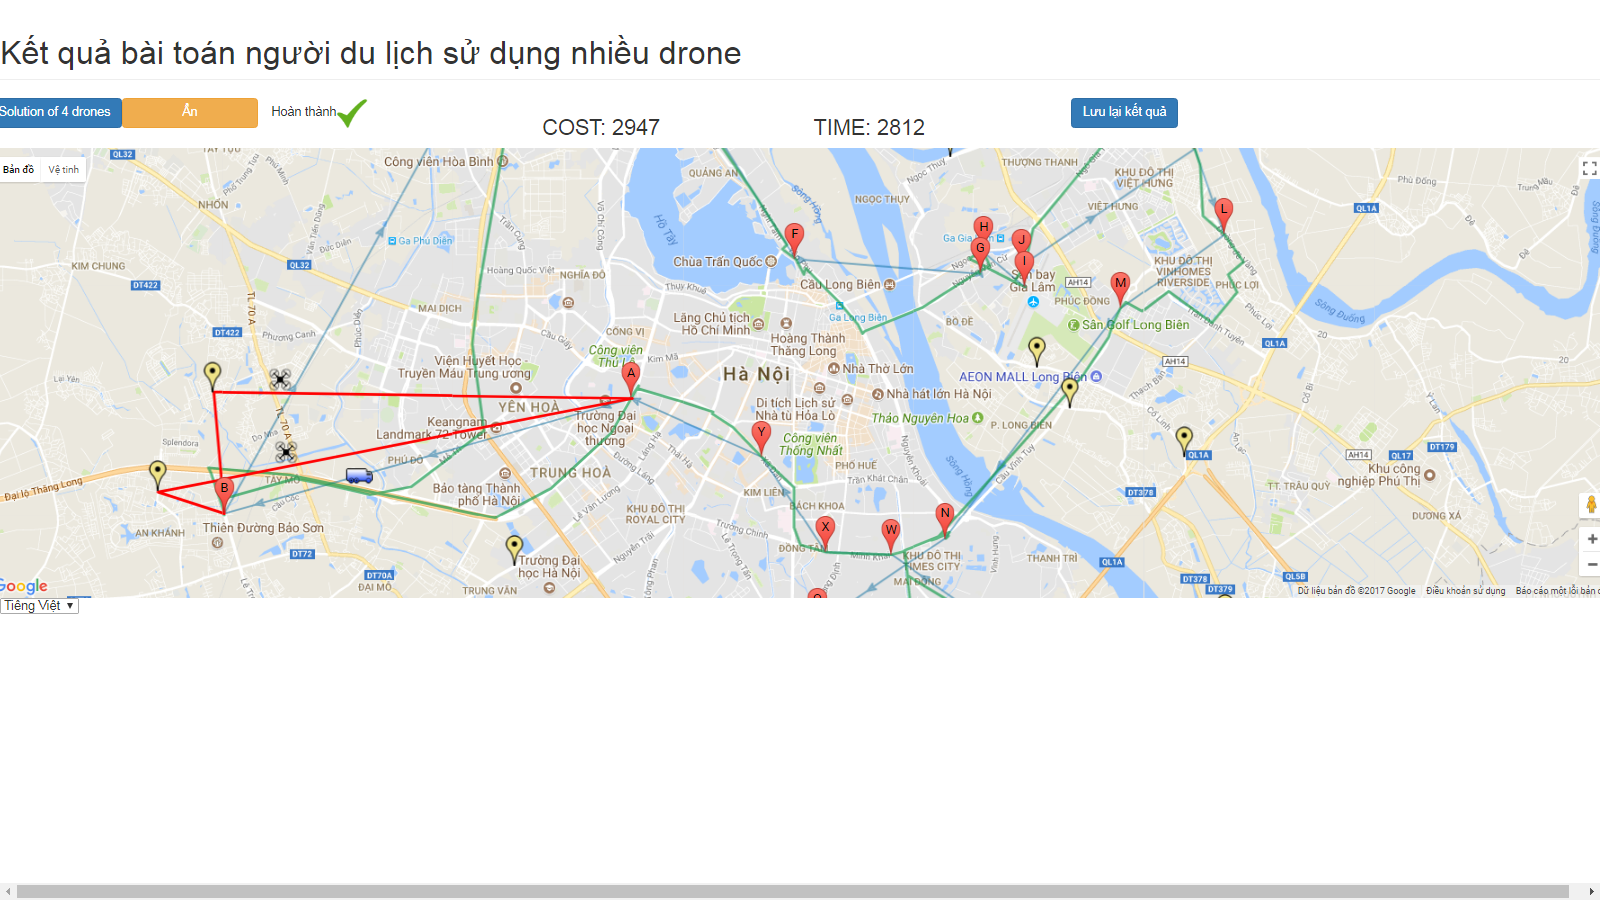
\includegraphics[scale=0.25]{screen/solution2.png}
\caption{Màn hình kết quả với bốn drone}
\label{solution2}
\end{figure}
\end{frame}
\begin{frame}{Video Demo}
\begin{figure}[ht]
\includemovie[poster,autoplay,externalviewer, text={\small(Loading sample.avi)}]{6cm}{6cm}{video.mp4}
\end{figure}

\end{frame}
\begin{frame}[plain]{Thank you for attention!}

\includegraphics[scale=0.7]{camon.jpg}
\end{frame}

\end{document}
